As for a start, we computed and compared the solutions at time of $t = \pi$.\\
The exact and numerical solutions are summarised in figure 6.1. In figure 6.1 the numerical solutions shown were computed using $Pm\,1\,(b)$ with grid size $60 \times 60$ ($CFL = 0.1$) just for a qualitative visualisation. According to the Figure 6.1, the numerical results do seem to be a good approximation to the exact solution in terms of shape and structure. However they do differ in magnitude and especially for pressure. One of the appropriate explanation is because we are comparing the solutions at time = $\pi$ and this actually makes the analytical solutions all equal to 0! In Python (32 bit) 0 is represented by random numbers with a magnitude about $10^{-17}$. Hence truncation errors caused by 0 might overruns the time discretisation error. Besides this, for pressure we are actually comparing solution at $n-\dfrac{1}{2}$ step ($n$ is the total time step). Hence the the final time is not $\pi$ but rather equals to $\pi - 0.5\Delta t$. Therefore the final time depends on the size of $\Delta t$ too which also makes the approximation worse. In this case with $CFL = 0.1$ we have the final time equals $3.13833$. We infer that the accuracy should improve for small $CFL$ numbers so that the final time for pressure is close to $\pi$. This is confirmed by the more consistent 2nd order convergence rates shown in Figure 6.2 where $CFL = 0.05$ was used.\\
Talk about the error behaviour for Pm 1 (a)!

We observed large numerical boundary layer in pressure error for $Pm\,1\,(a)$. This is because of the inconsistent normal pressure gradient. For $Pm\,1\,(b)$ where the more consistent update formula is used shows a much reduced numerical boundary layer in pressure error.
%_________________________________

Because we have observed that the error in velocities are almost identical to each other in all test runs, hence only the results of $U$ velocities are presented here.\\
As indicated by Figure 6.2 (a), the convergence error in velocities show fully 2nd order rate. This result is also consistent across all norms ($L_1,\,L_2\,L_\infty$). In fact we observed fully 2nd order convergence rates for velocity in all test runs. This implies that the spurious mode contained in the intermediate velocity field is successfully filtered out by the update formula ($\textbf{u}^{n+1} = \textbf{u}^* - \Delta t \nabla \phi^{n+1}$). This matches with the result in literature too \cite{brown2001accurate,guermond2004error,guermond2006overview}.\\

The results in pressure is however not completely satisfied. Even though the $L_2$ and $L_\infty$ rates show close to 2nd convergence rates ($L_2 = 1.8004$ and $L_\infty = 1.8000$), $L_1$ showed a deteriorated rate of 1.6692. The exact cause of this deterioration in accuracy remains unknown. One possible explanation is because we are comparing solutions at at time very close to $\pi$ ($t = 3.141$ with $CFL = 0.05$), then the truncation error caused by 0 might start to dominate especially for finer grids. This is supported by the table of convergence rates shown in Table 6.1 where rates decreases rapidly at finer grids. However this explanation is still not satisfied as it cannot explain why we observed consistent 2nd order rate in velocity from coarse to fine grids.\\

Nevertheless, it really suggest that we should avoid computing solutions at such a $t$.

\begin{figure}[H]
	\centering
	\begin{subfigure}[t]{2.5in}
		\centering
		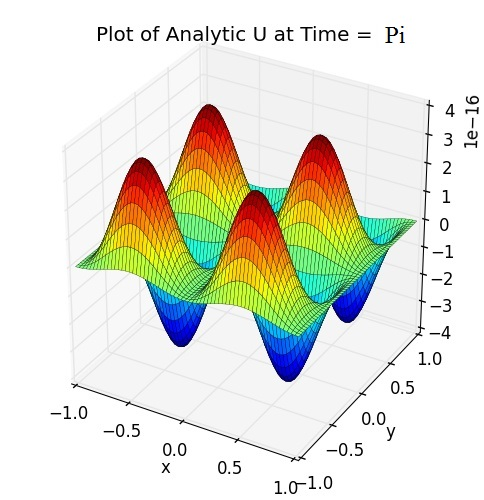
\includegraphics[width=2.5in]{figures/Pm1b_pf2_U_exact_t_pi_grid_60.jpg}
		\caption{Analytic $U$ velocity at $t=\pi$}\label{fig:6.1a}		
	\end{subfigure}
	\quad
	\begin{subfigure}[t]{2.5in}
		\centering
		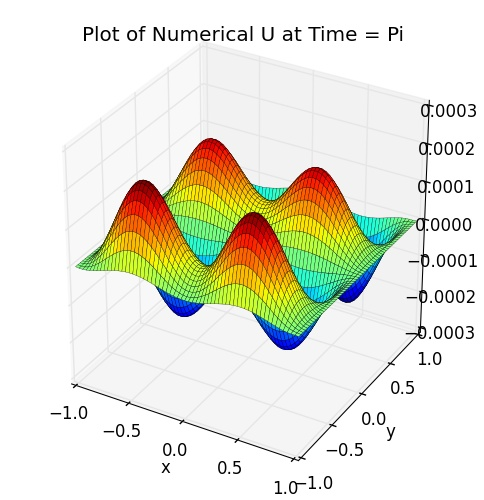
\includegraphics[width=2.5in]{figures/Pm1b_pf2_uf_t_pi_grid_60_0_05.jpg}
		\caption{Numerical $U$ velocity at $t=\pi$}\label{fig:6.1b}
	\end{subfigure}
	\quad
	\begin{subfigure}[t]{2.5in}
		\centering
		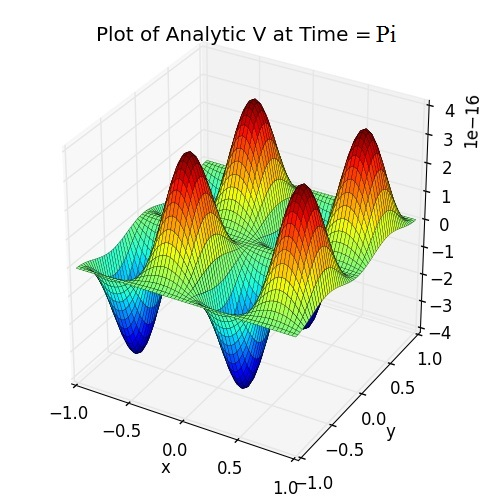
\includegraphics[width=2.5in]{figures/Pm1b_pf2_V_exact_t_pi_grid_60.jpg}
		\caption{Analytic $V$ velocity at $t=\pi$}\label{fig:6.1b}
	\end{subfigure}
	\quad
	\begin{subfigure}[t]{2.5in}
		\centering
		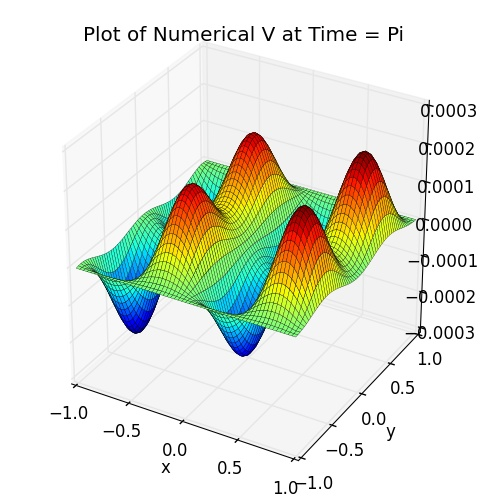
\includegraphics[width=2.5in]{figures/Pm1b_pf2_vf_t_pi_grid_60_0_05.jpg}
		\caption{Numerical $V$ velocity at $t=\pi$}\label{fig:6.1b}
	\end{subfigure}
	\quad	
	\begin{subfigure}[t]{2.5in}
		\centering
		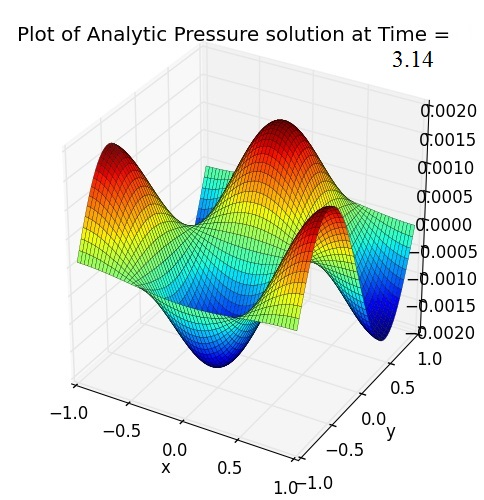
\includegraphics[width=2.5in]{figures/Pm1b_pf2_P_exact_t_pi_grid_60_cfl_0_1.jpg}
		\caption{Analytic pressure ($P$) at $t=3.14$}\label{fig:6.1b}
	\end{subfigure}
	\quad	
	\begin{subfigure}[t]{2.5in}
		\centering
		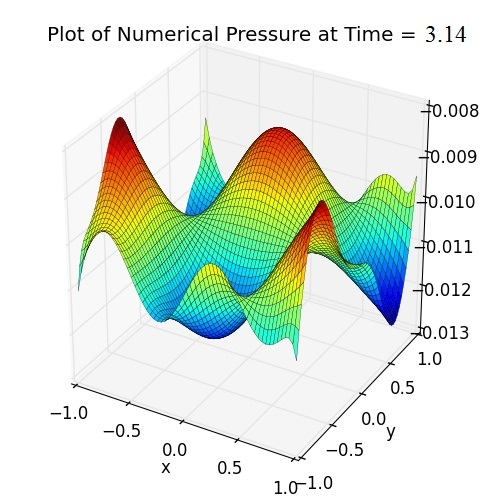
\includegraphics[width=2.5in]{figures/Pm1b_pf2_pf_t_pi_grid_60_cfl_0_1.jpg}
		\caption{Numerical pressure ($P$) at $t=3.14$}\label{fig:6.1b}
	\end{subfigure}
	\caption{Plot of exact solutions ($U,V,P$) at time $\pi$ on the spatial domain of $[-1,1]^2$ with grid size $60 \times 60$ and $CFL=0.1$}\label{fig:6.1}
\end{figure}

\begin{figure}[H]
	\centering
	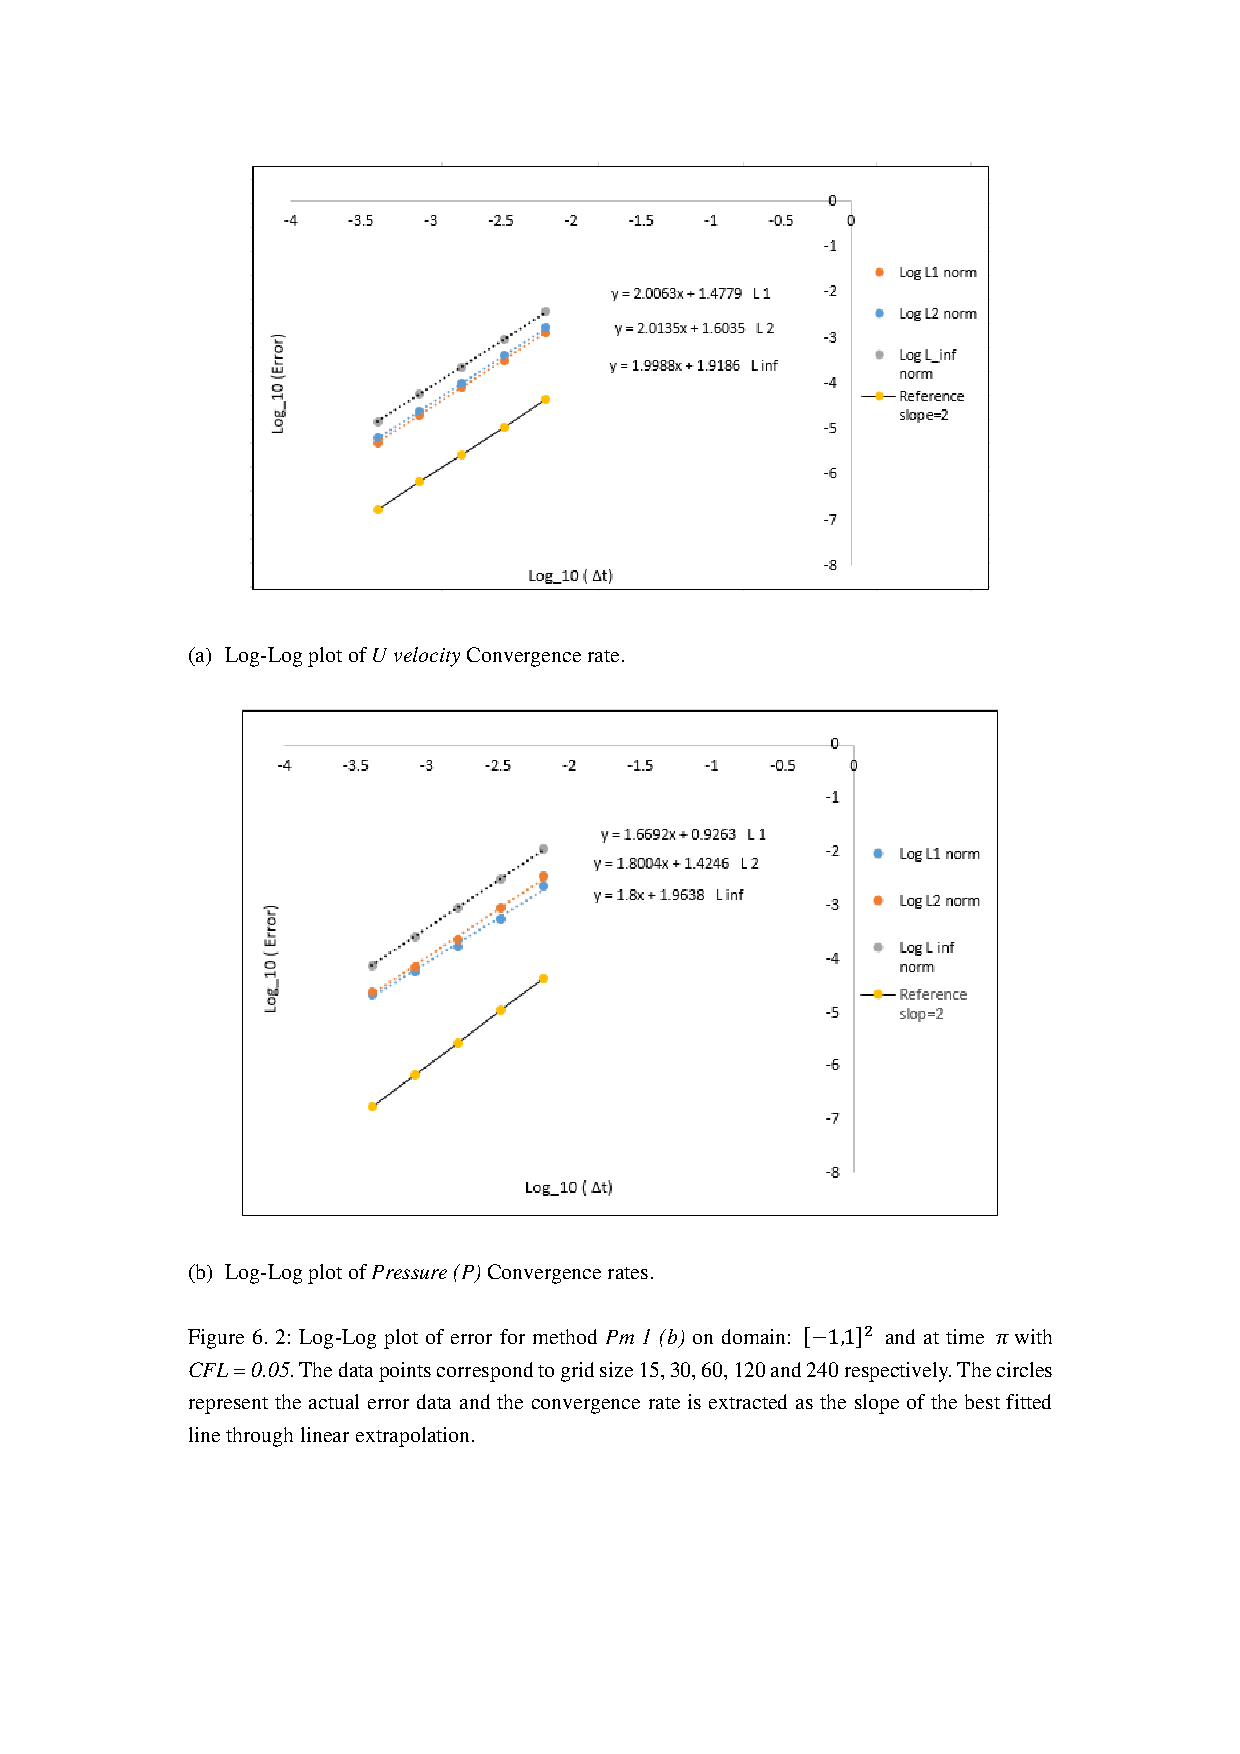
\includegraphics[scale=0.9]{figures/Pm1b_pf2_rate_t_pi_grid_60_cfl_0_05.pdf}
	\caption{Log-Log plot of error for method Pm 1 (b) on domain: [-1,1]^2 and at time π with CFL = 0.05. The data points correspond to grid size 15, 30, 60, 120 and 240 respectively. The circles represent the actual error data and the convergence rate is extracted as the slope of the best fitted line through linear extrapolation.}\label{fig:6.2}
\end{figure}

\newpage
\begin{table}	
\centering
\begin{tabular}{|l|l|l|l|l|}
	\hline
	U Velocity & Rate for grid: 15 - 30 & 30 - 60 & 60 - 120 & 120 - 240\\
	\hline
	$L_1$ & 2.004 & 2.012 & 2.005 & 2.002\\
	$L_2$ & 2.042 & 2.012 & 2.004 & 2.001\\
	$L_\infty$ & 2.009 & 1.988 & 2.001 & 2.000\\
	\hline
	P Pressure &  Rate for grid: 15 - 30 & 30 - 60 & 60 - 120 & 120 - 240\\
	\hline
	$L_1$ & 2.061 & 1.717 & 1.518 & 1.432\\
	$L_2$ & 2.039 & 1.898 & 1.713 & 1.548\\
	$L_\infty$ & 1.886 & 1.752 & 1.795 & 1.793\\
	\hline
\end{tabular}
\caption{Convergence rates for method $Pm\,1\,(b)$ on domain: $[-1,1]^2$ and time $\pi$. The rates were calculated taking the logarithm of the ratio of errors between 2 consecutive grids}\label{table:1}
\end{table}


\begin{figure}[H]
	\centering
	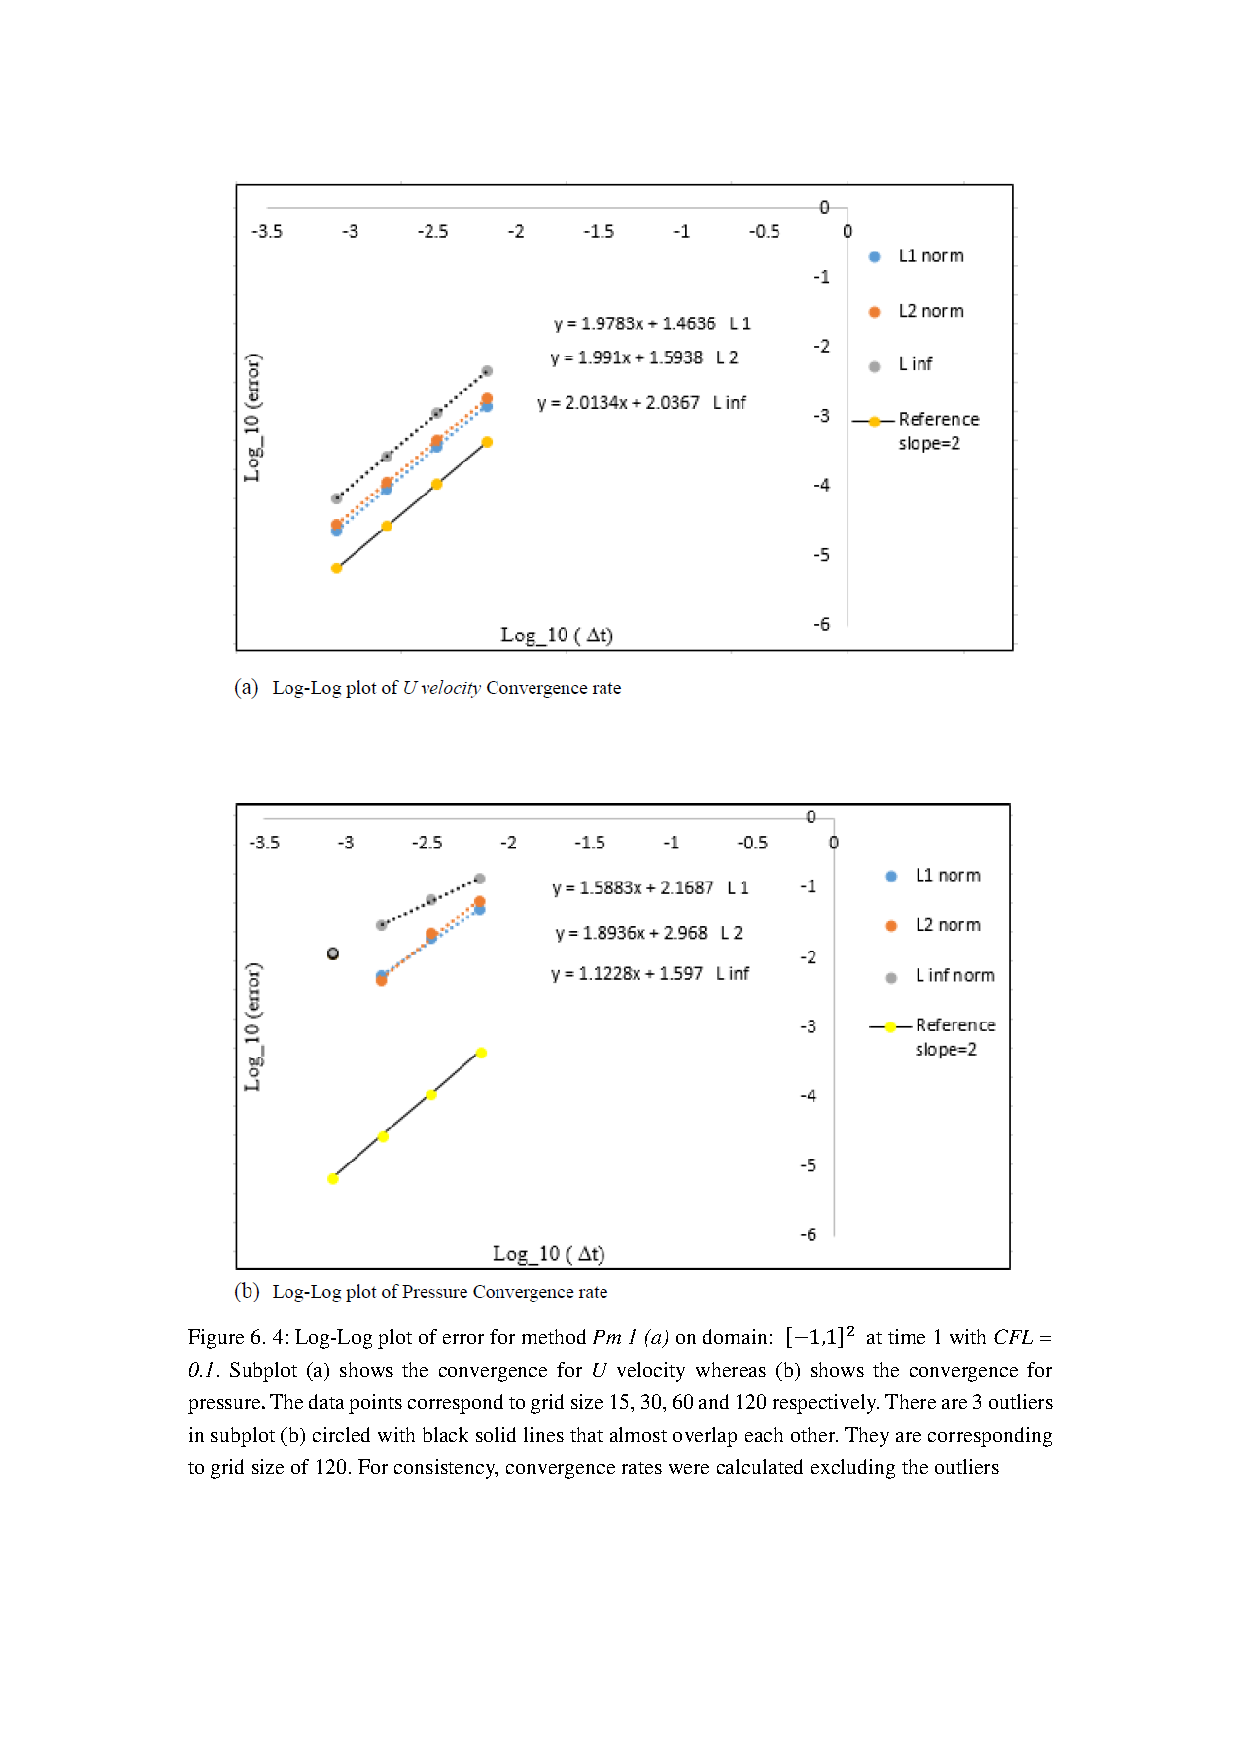
\includegraphics[scale=0.9]{figures/Pm1a_pf2_rate_t_1_cfl_0_5.pdf}
	\caption{Log-Log plot of error for method \textit{Pm 1 (a)} on domain: $[-1,1]^2$ and at time 1 with CFL = 0.5. Subplot (a) shows the convergence for U velocity whereas (b) shows the convergence for pressure and (c) for $\nabla \cdot \textbf{u}^*$. The data points correspond to grid size 15, 30, 60 and 120 respectively. In subplot (b), there are 3 outliers (two almost overlapped each other) for each norm at grid size 120. They are represented as circles with black solid lines.}\label{fig:6.4}
\end{figure}

\begin{figure}[H]
	\centering
	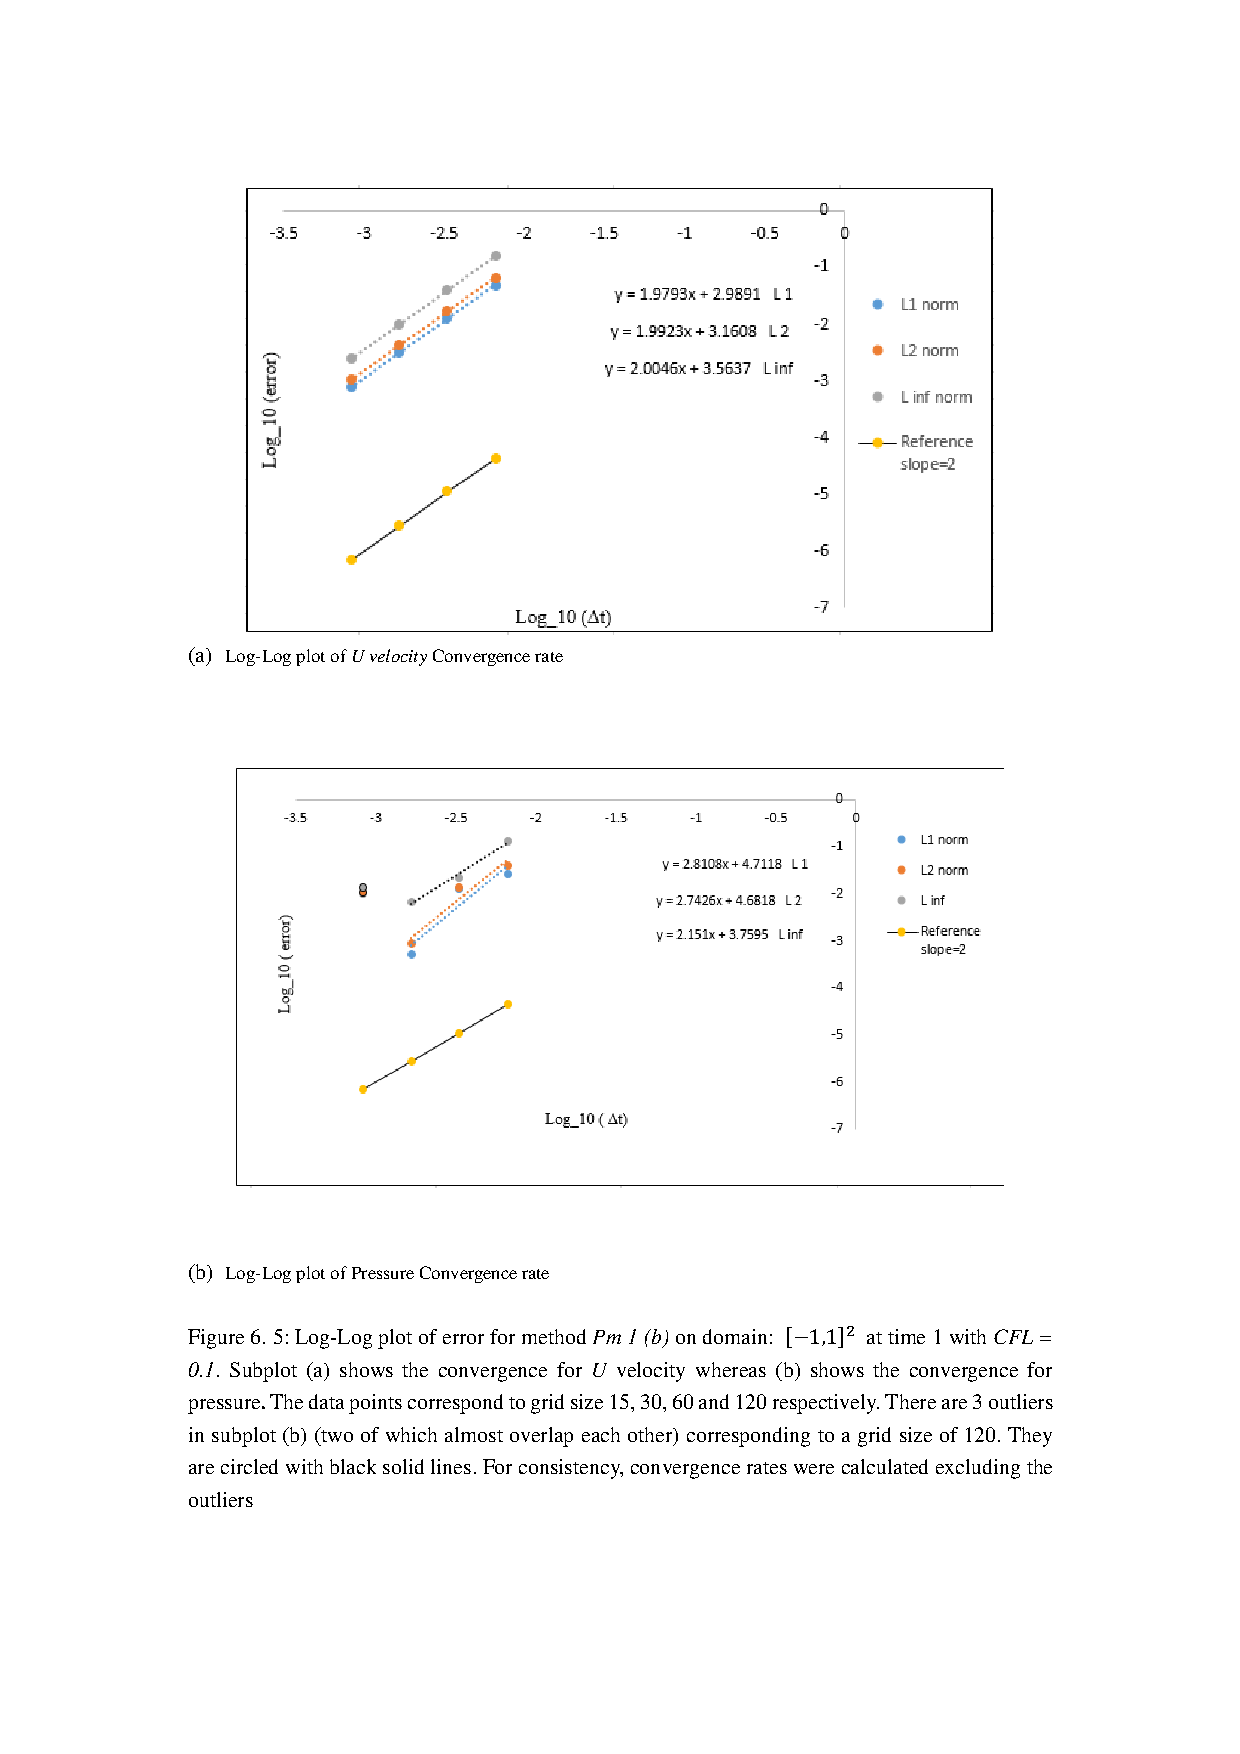
\includegraphics[scale=0.9]{figures/Pm1b_pf2_rate_t_1_cfl_0_5.pdf}
	\caption{Log-Log plot of error for method \textit{Pm 1 (a)} on domain: $[-1,1]^2$ and at time 1 with CFL = 0.5. Subplot (a) shows the convergence for U velocity whereas (b) shows the convergence for pressure and (c) for $\nabla \cdot \textbf{u}^*$. The data points correspond to grid size 15, 30, 60 and 120 respectively. In subplot (b), there are 3 outliers (two almost overlapped each other) for each norm at grid size 120. They are represented as circles with black solid lines.}\label{fig:6.5}
\end{figure}

\begin{figure}[H]
	\centering
	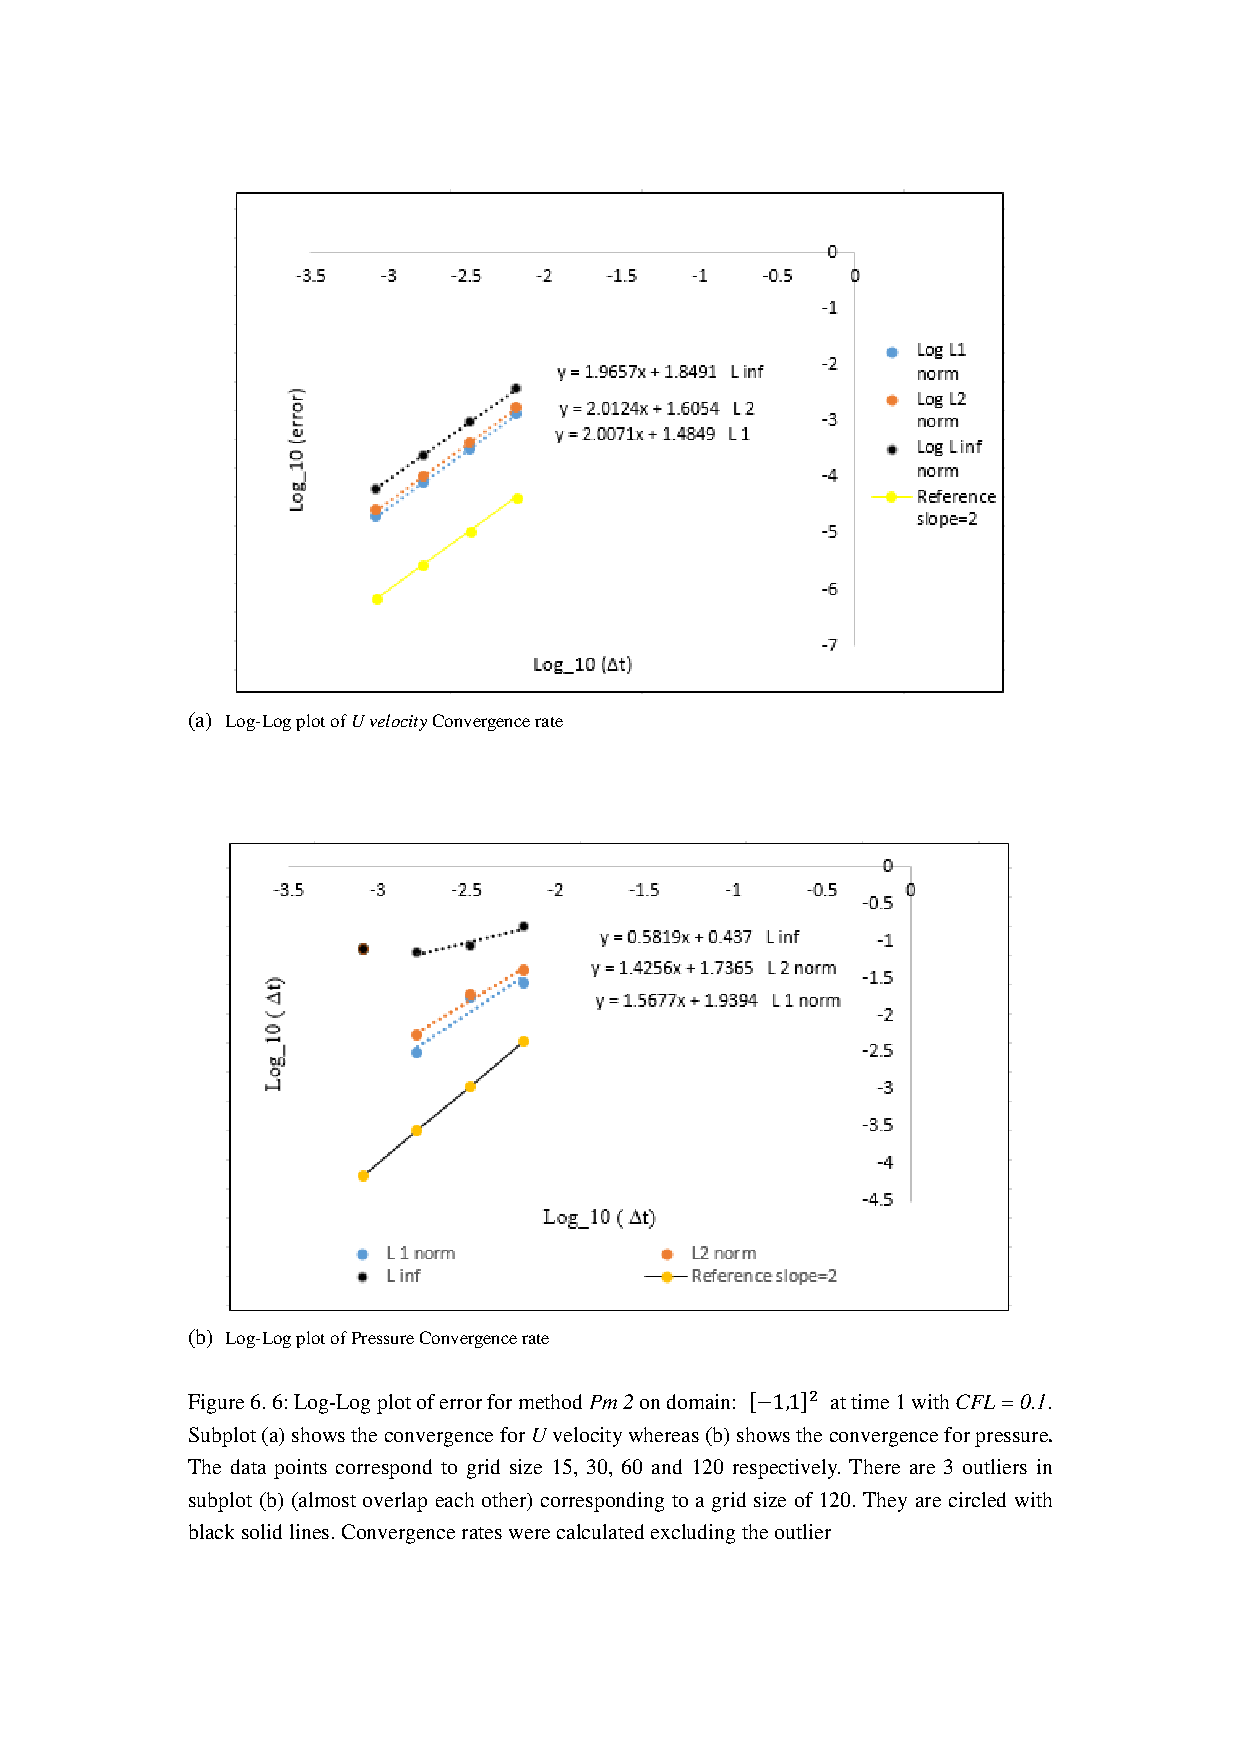
\includegraphics[scale=0.9]{figures/Pm2_pf2_rate_t_1_cfl_0_1.pdf}
	\caption{Log-Log plot of error for method \textit{Pm 1 (a)} on domain: $[-1,1]^2$ and at time 1 with CFL = 0.5. Subplot (a) shows the convergence for U velocity whereas (b) shows the convergence for pressure and (c) for $\nabla \cdot \textbf{u}^*$. The data points correspond to grid size 15, 30, 60 and 120 respectively. In subplot (b), there are 3 outliers (two almost overlapped each other) for each norm at grid size 120. They are represented as circles with black solid lines.}\label{fig:6.6}
\end{figure}

\begin{figure}[H]
	\centering
	\begin{subfigure}[t]{2.5in}
		\centering
		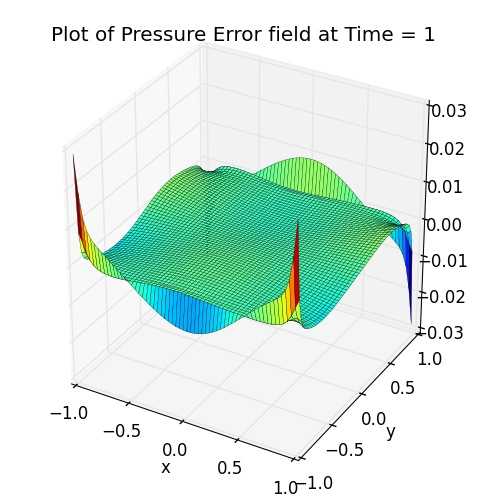
\includegraphics[width=2.5in]{figures/Pm1a_pf2_P_error_t_1_grid_60_cfl_0_1.jpg}
		\caption{Pressure error field for method $Pm\,1\,(a)$}\label{fig:6.7a}		
	\end{subfigure}
	\quad
	\begin{subfigure}[t]{2.5in}
		\centering
		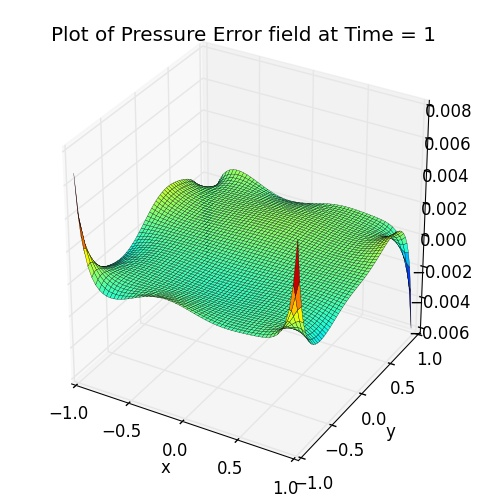
\includegraphics[width=2.5in]{figures/Pm1b_pf2_P_error_t_1_grid_60_cfl_0_1.jpg}
		\caption{Pressure error field for method $Pm\,1\,(b)$}\label{fig:6.7b}
	\end{subfigure}
	\caption{Plot of Pressure error field on the spatial domain of $[-1,1]^2$ at time $t=1$ with grid size of $60 \times 60$. A CFL number of 0.1 was used.}\label{fig:6.7}
\end{figure}

\begin{figure}[H]
	\centering
	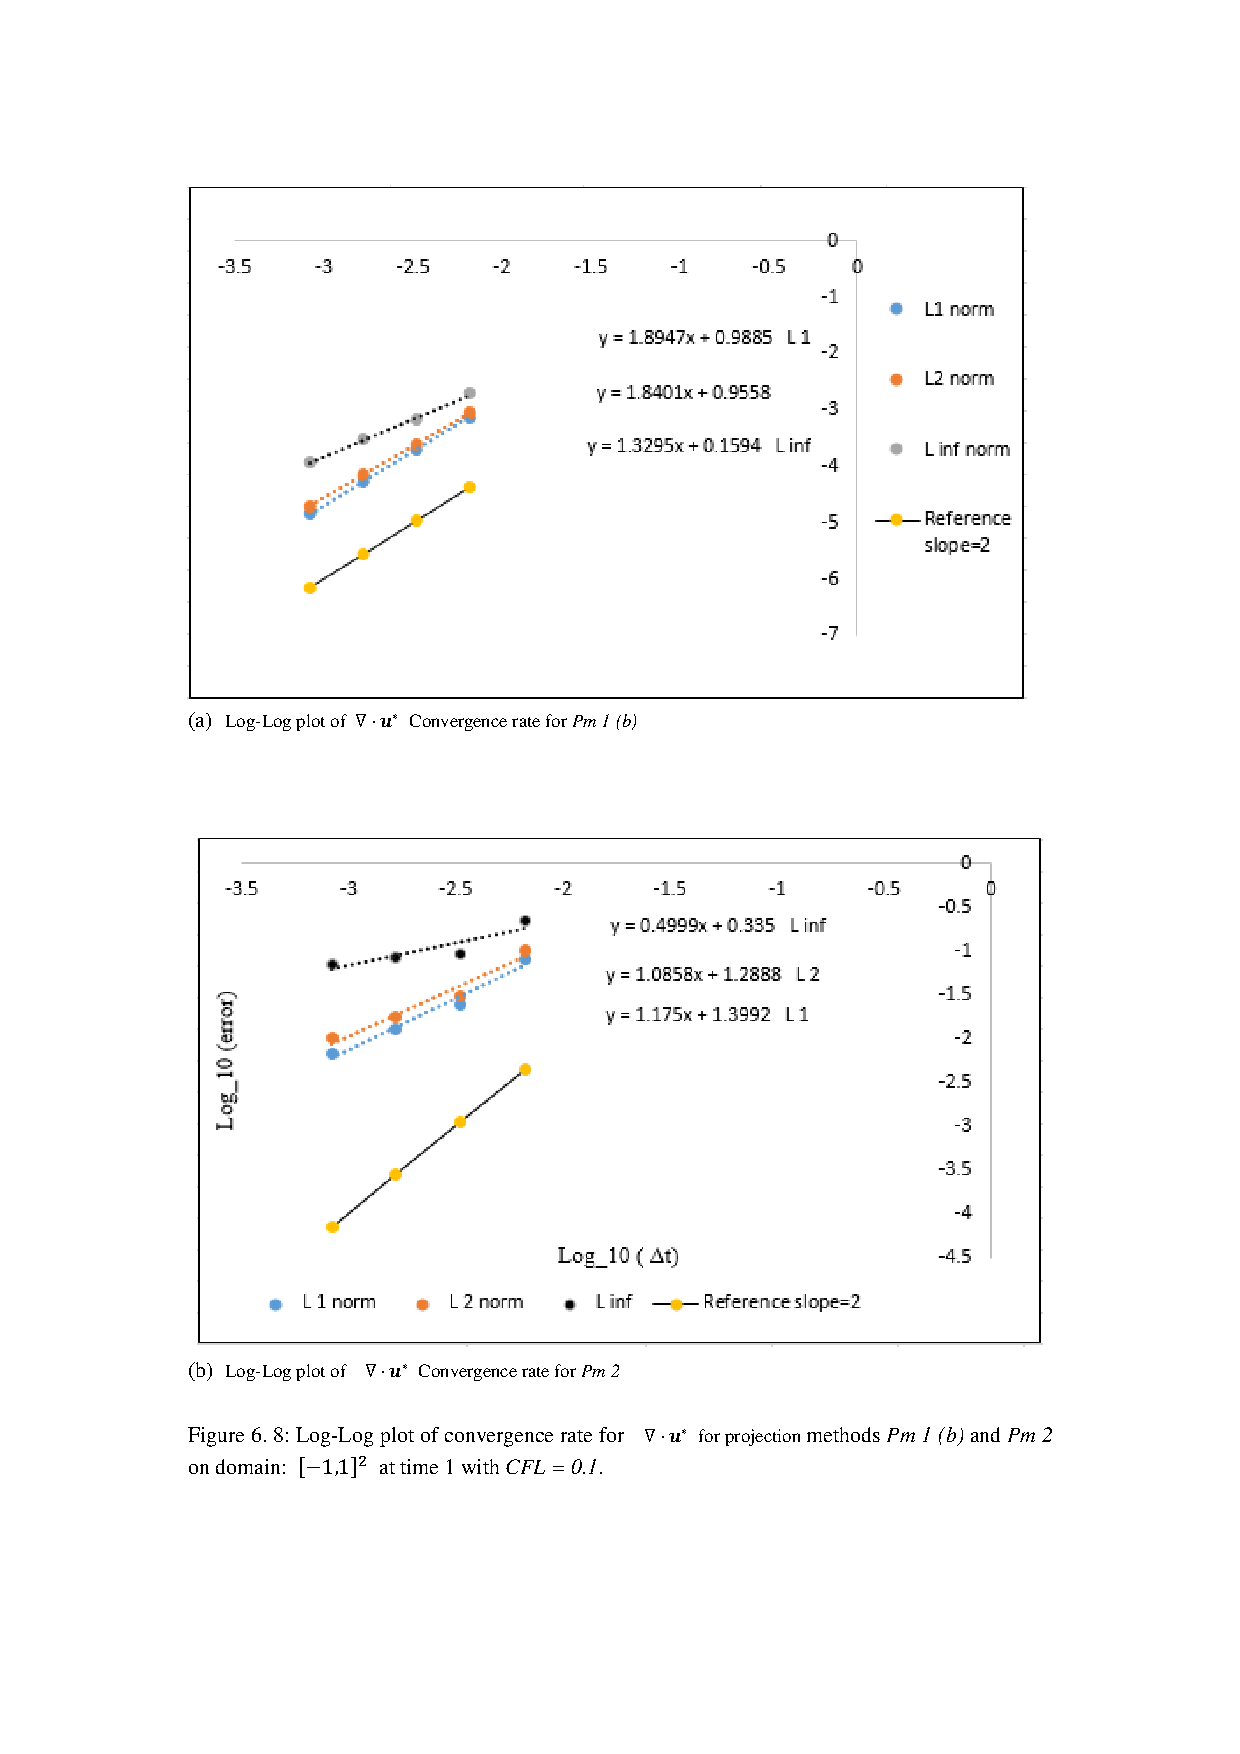
\includegraphics[scale=0.9]{figures/Pm2_Pm1b_div_uvstar_rate_t_1_cfl_0_1.pdf}
	\caption{Log-Log plot of convergence rate for $\nabla \cdot \textbf{u}^*$ for projection methods Pm 1 (b) and Pm 2 on domain: [-1,1]^2 at time 1 with CFL = 0.1. }\label{fig:6.8}
\end{figure}

\begin{figure}[H]
	\centering
	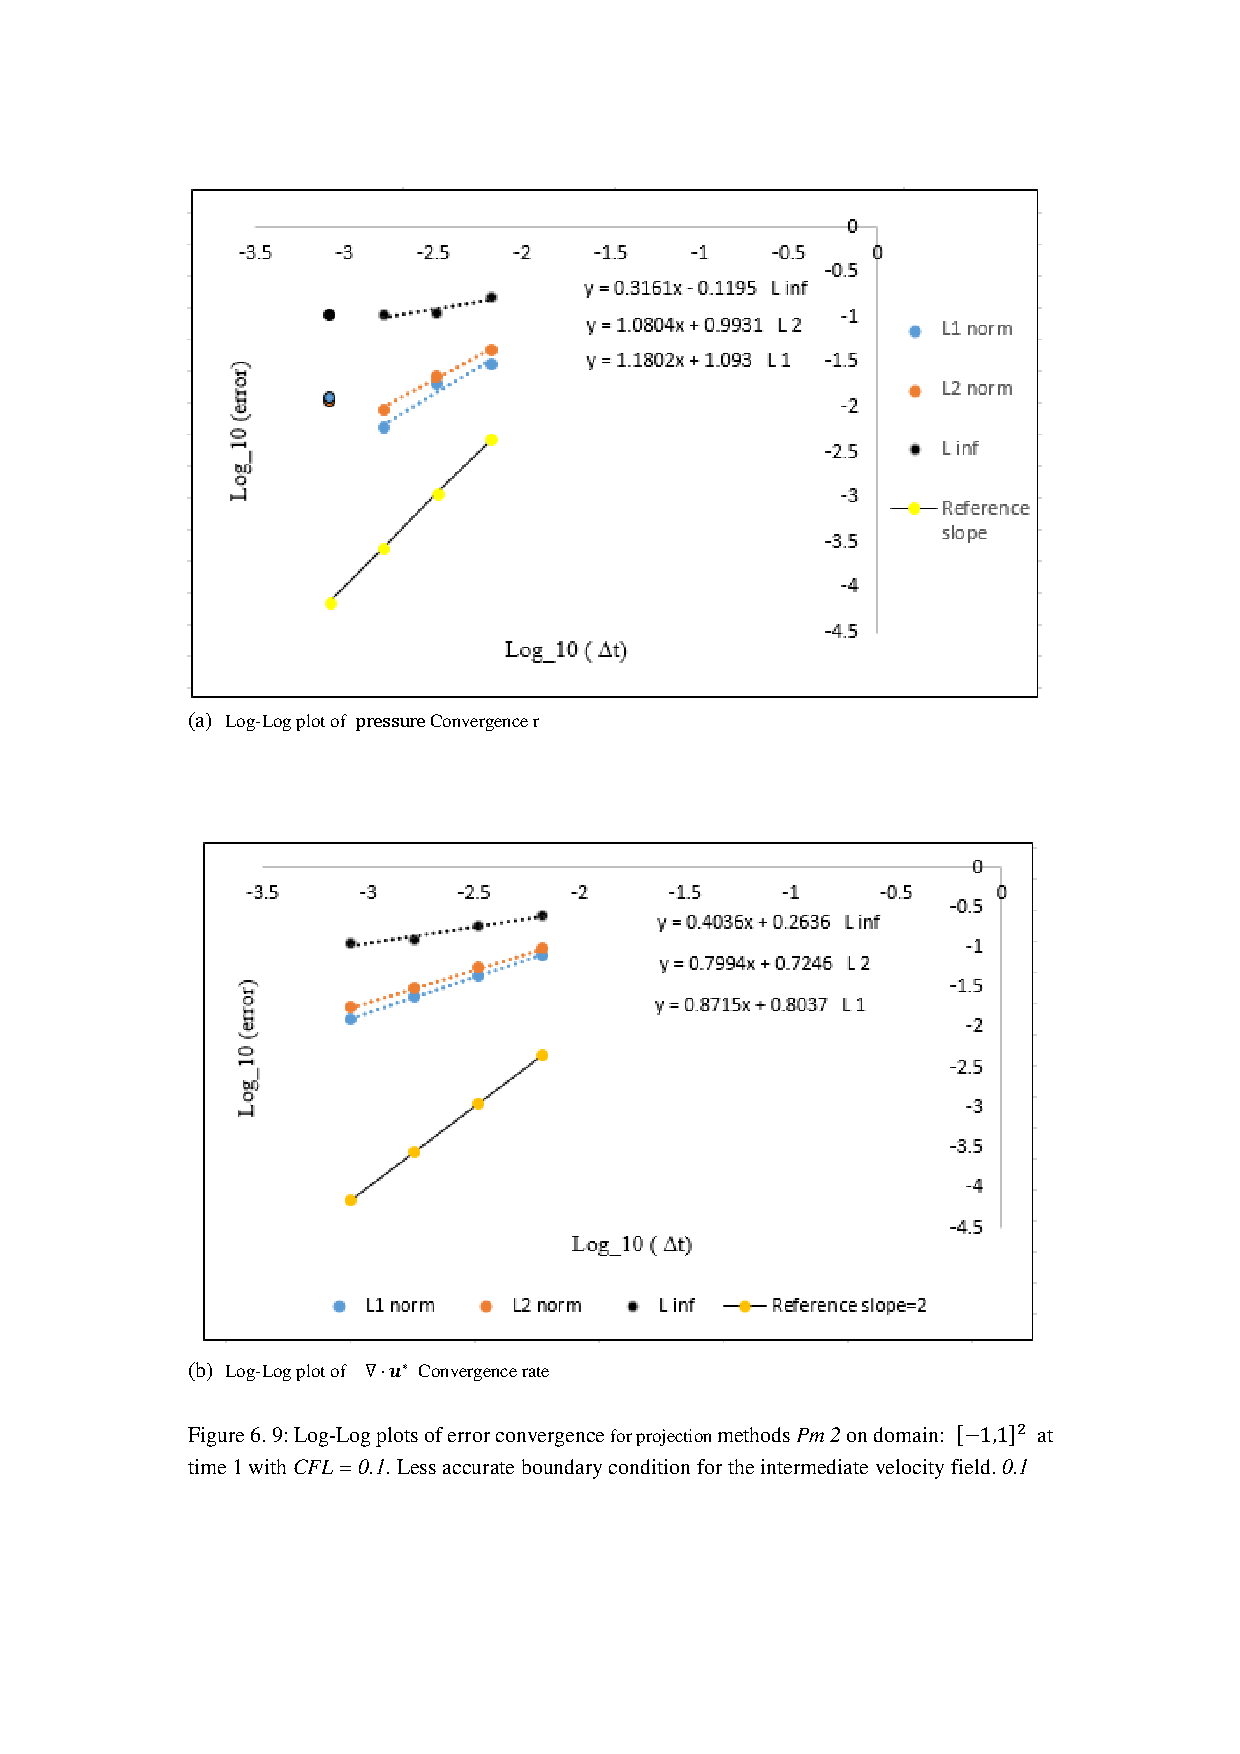
\includegraphics[scale=0.9]{figures/Pm2_2_rate_t_1_cfl_0_1.pdf}
	\caption{Log-Log plot of convergence rate for $\nabla \cdot \textbf{u}^*$ for projection methods Pm 1 (b) and Pm 2 on domain: [-1,1]^2 at time 1 with CFL = 0.1. }\label{fig:6.9}
\end{figure}

\begin{figure}[H]
	\centering
	\begin{subfigure}[t]{2.5in}
		\centering
		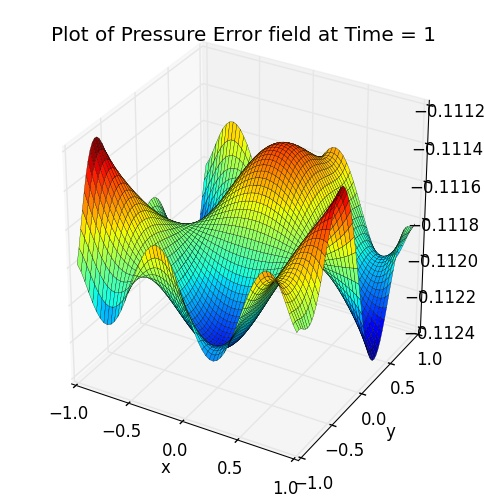
\includegraphics[width=2.5in]{figures/Pm2_pf2_P_error_t_1_grid_60.jpg}
		\caption{Pressure error field for method $Pm\,2$}\label{fig:6.10a}		
	\end{subfigure}
	\quad
	\begin{subfigure}[t]{2.5in}
		\centering
		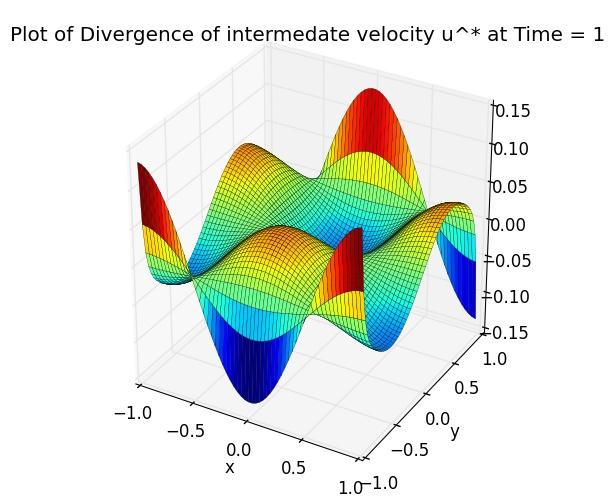
\includegraphics[width=2.5in]{figures/Pm2_pf2_div_uvstar_t_1_grid_60.jpg}
		\caption{$3D$ surface plot of $\nabla \cdot \textbf{u}^*$ of method $Pm\,2$}\label{fig:6.10b}
	\end{subfigure}
	\caption{Plot of Pressure error field and $\nabla \cdot \textbf{u}^*$ for $Pm\,2$ on the spatial domain of $[-1,1]^2$ and at time $t=1$ with grid size of $60 \times 60$. A CFL number of 0.1 was used.}\label{fig:6.10}
\end{figure}

Let's take a look at the Gauge method (see Figure 6.11) the error in both velocity and pressure shows fully second order accuracy. However outliers were once again observed at finer grids (grid size 120) too. This indicating that the Gauge methods also suffers from this error enlargement at finer grids. The plot of error field shows that the error is more smooth along the boundary. This might explain the improve in accuracy (for small to moderate grid)

\begin{figure}[H]
	\centering
	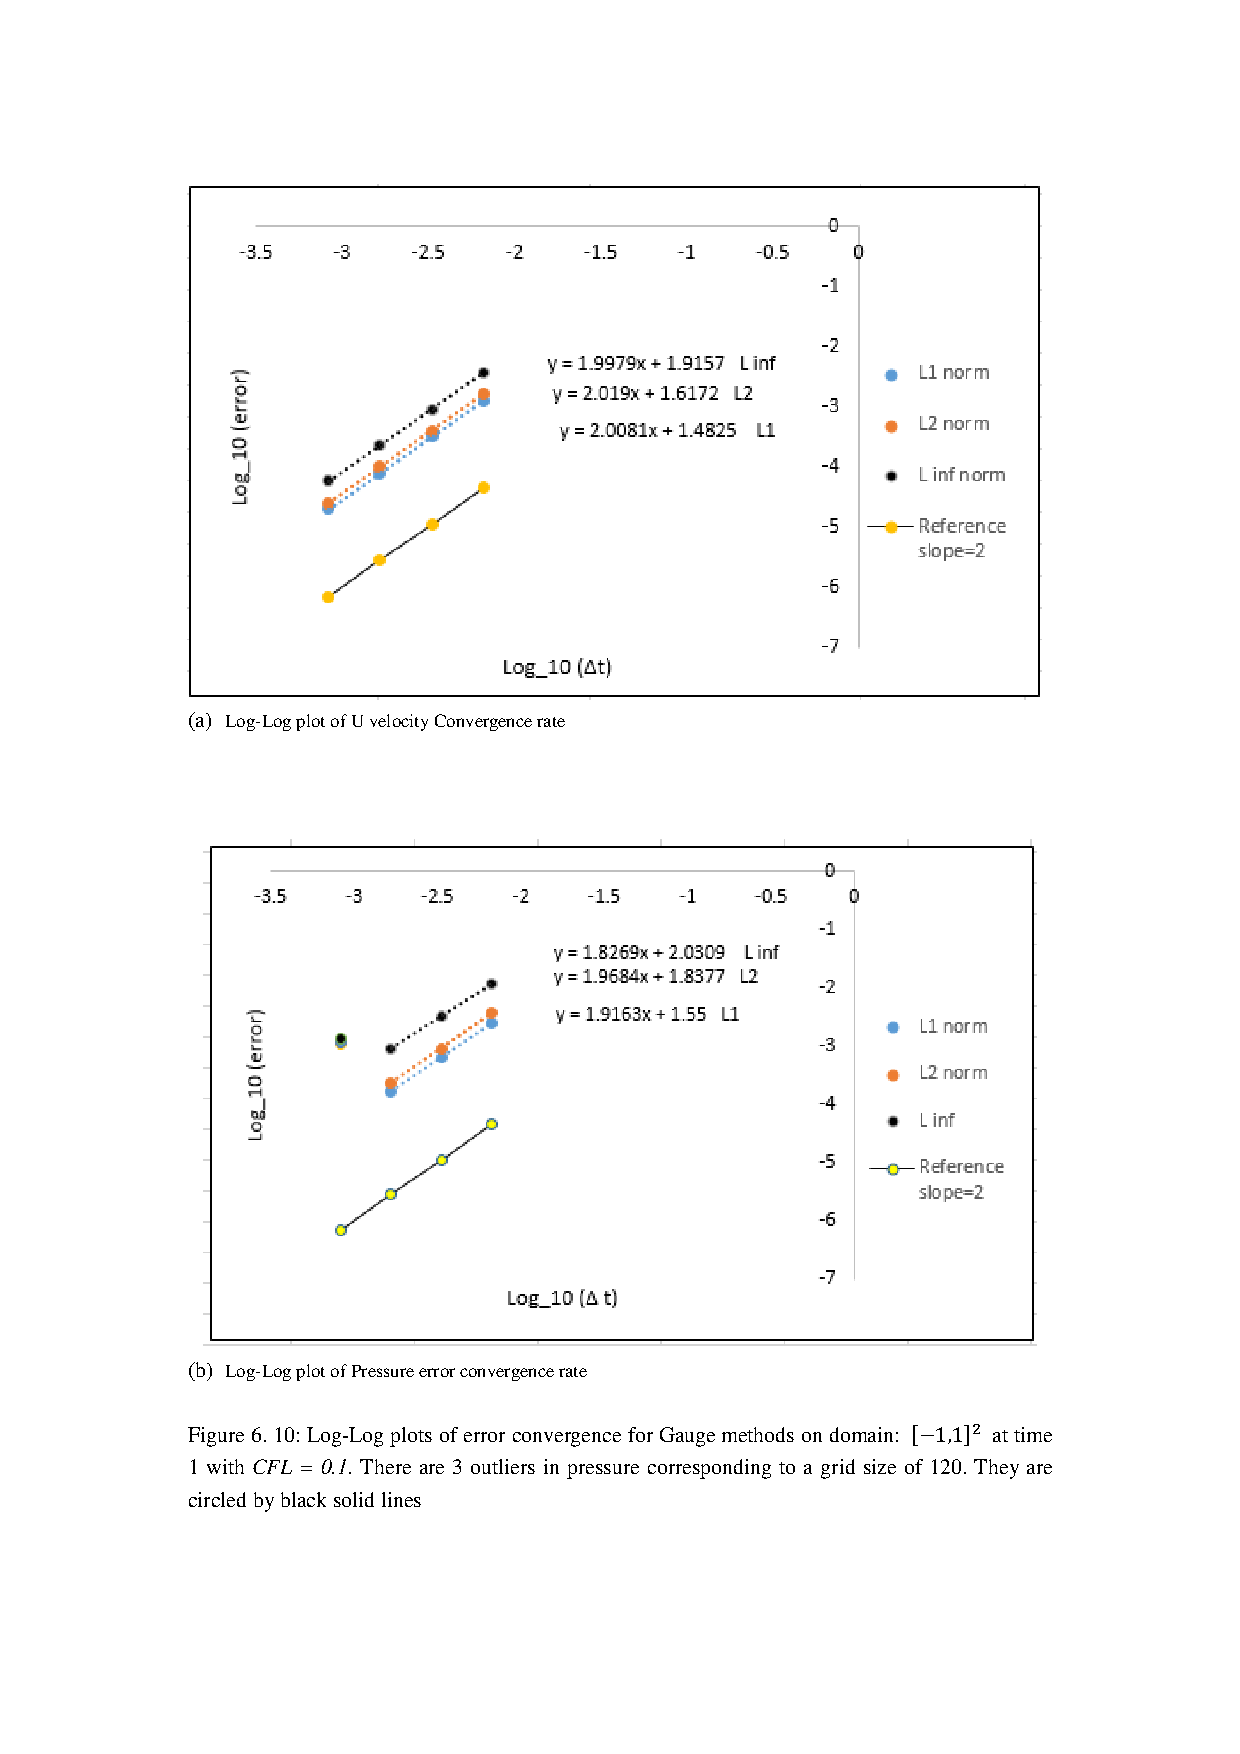
\includegraphics[scale=0.9]{figures/Gauge_pf2_rate_t_1_cfl_0_1.pdf}
	\caption{Log-Log plot of convergence rate for pressure and velocity of the Gauge method on the spatial domain: $[-1,1]^2$ and at time 1 with CFL = 0.1. }\label{fig:6.11}
\end{figure}

\begin{figure}[H]
	\centering
	\begin{subfigure}[t]{2.5in}
		\centering
		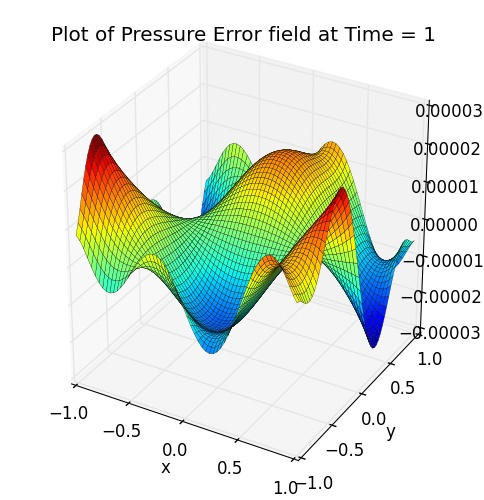
\includegraphics[width=2.5in]{figures/Gauge_pf2_P_error_t_1_grid_60.jpg}
		\caption{Pressure error field for Gauge method}\label{fig:6.12a}		
	\end{subfigure}
	\quad
	\begin{subfigure}[t]{2.5in}
		\centering
		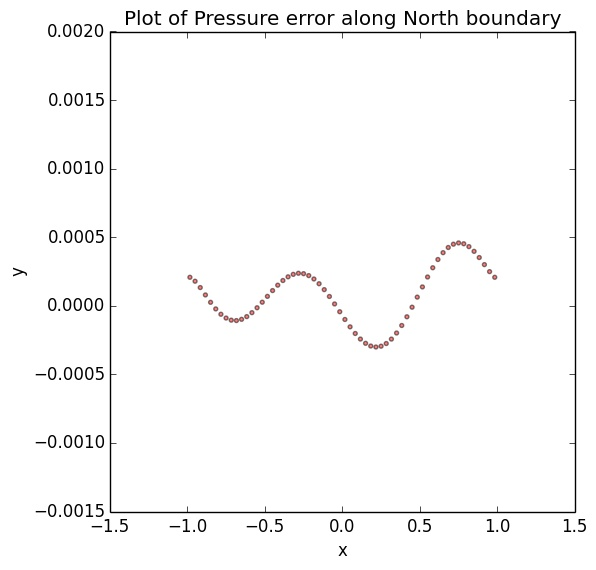
\includegraphics[width=2.5in]{figures/Gauge_pf2_N_P_error_t_1_grid_60.jpg}
		\caption{Plot of Pressure error at North boundary ($y=1$)}\label{fig:6.12b}
	\end{subfigure}
	\quad
	\begin{subfigure}[t]{2.5in}
		\centering
		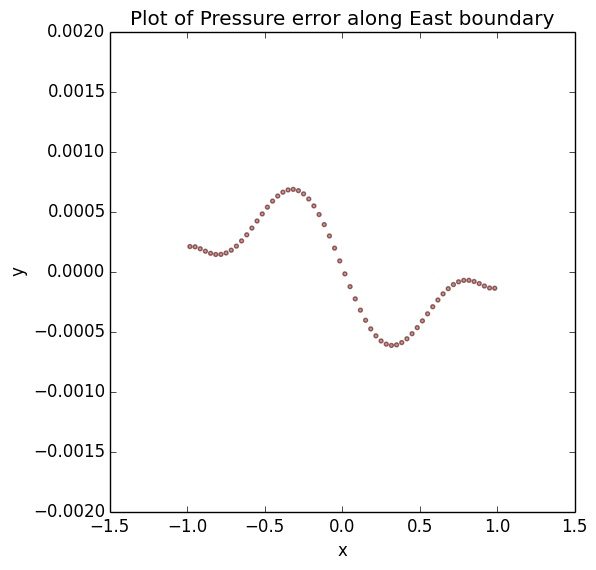
\includegraphics[width=2.5in]{figures/Gauge_pf2_E_P_error_t_1_grid_60.jpg}
		\caption{Plot of Pressure error at East boundary ($x=1$)}\label{fig:6.12c}
	\end{subfigure}
	\caption{Plot of Pressure error field for Gauge method on the spatial domain of $[-1,1]^2$ and at time $t=1$ with grid size of $60 \times 60$. A CFL number of 0.1 was used. The error plot for Sourth and West boundaries are similar hence not presented here.}\label{fig:6.12}
\end{figure}

%______________________________
\textbf{GOES to IMPLEMENTATION!}
\newpage
Our results presented above does show good of alignment with those published in the literature. However it is a bit disappointed because they are limited to small to moderate grids (grid size 15 to 60). At such a ``small" grid size, not only the fluid flow problem is made much less interesting, but also affects the accuracy in a negative way. Recall we are interested in examining the convergence in temporal error but the actual error between numerical and analytic solution is consisted of both spatial and temporal errors. \\
For second order accuracy schemes the error is
\begin{equation}
e_h = \mathcal{O}(\Delta x^2) + \mathcal{O}(\Delta t^2)
\end{equation}
At small grid sizes the spatial error ($\mathcal{O}(\Delta x^2)$) is large and hence dominate the overall error. This in turn makes our accuracy test of temporal errors less reliable.\\ Therefore to obtain optimal results and hence better error analysis we really want to push the numerical solvers up to handle fine grids.\\

However it is not so straightforward to do it and the reason why our numerical solver fails still remains puzzling.\\

To investigate the problem further, let's consider the projection method $Pm\,1\,(b)$ again on the spatial domain of $[-1,1]^2$. Because the increasing error behaviour occurs in pressure, hence let's re-examine the update formula
\begin{equation*}
p^{n+1/2} = p^{n-1/2} + \phi^{n+1} - \dfrac{\Delta t}{2\,Re}\,\nabla^2 \phi^{n+1} = p^{n-1/2} + \phi^{n+1} - \dfrac{1}{2\,Re}\,\nabla \cdot \textbf{u}^*
\end{equation*}
The numerical pressure calculated this way has a strong dependence or the accuracy of the auxiliary field $\phi^{n+1}$ and the divergence of the intermediate velocity $\textbf{u}^*$. Hence we first infer that the increase of error at finer grids are likely due to either the poor convergence in $\phi^{n+1}$ or $\nabla \cdot \textbf{u}^*$. To test our hypothesis let's take a look at the convergence rates of these variables which are summarised in Table 6.2. \\
Although the intermediate velocity field is not divergence free (at least it is not forced to be as in the case of $\textbf{u}^{n+1}$), it is however a good approximation to $\textbf{u}^{n+1}$. Hence it is natural to expect that the divergence of $\textbf{u}^*$ should converge to zero in the long runs too.\\

According to the data shown in Table 6.2, the errors in pressure jumped up significantly going from grid size 60 to 120 in all norms measured whereas other variables show consistent decreasing in errors. The complete convergence rates for these variables are included in Figure 6.5 (a) (b) and 6.8 (a) respectively. The fact that $\nabla \cdot \textbf{u}^*$ shows consistent convergence implies that the cause of strange error behaviour in pressure is rather caused by the auxiliary field $\phi^{n+1}$. In addition, the spurious mode contained in $\nabla \cdot \textbf{u}^*$ and $\phi^{n+1}$ is theoretically filtered out by the pressure update formula shown above. If this does not happen practically, the numerical boundary layer then formed should only degrade the error convergence (as we have seen in the error in $\nabla \cdot \textbf{u}^*$) not making it the errors enlarged in finer grids. This also cannot explain why we see good convergence in pressure for coarser grids since numerical boundary layers are an inherent property of projection methods independent of grid sizes. Nevertheless, we know that the problem must be caused by $\phi$\\

\begin{table}[H]
\centering
\begin{tabular}{|l|l|l|l|}
	\hline
	 $L_1$  \\
	 \hline
	 Grid size & Error in $U$ velocity & Error in Pressure & Error in $\nabla \cdot \textbf{u}^*$\\
	\hline
	30 & 1.23e-2 & 1.31e-2 & 2.04e-4\\
	60 & 3.11e-3 & 5.24e-4 & 5.39e-5\\
	120 & 7.78e-4 & 1.05e-2 & 1.41e-5\\
	\hline
	 $L_2$ \\
	\hline
	Grid size & Error in $U$ velocity & Error in Pressure & Error in $\nabla \cdot \textbf{u}^*$\\
	\hline
	30 & 1.69e-2 & 1.32e-2 & 2.49e-4\\
	60 & 4.23e-3 & 8.85e-4 & 7.01e-5\\
	120 & 1.06e-3& 1.05e-2 & 1.95e-5\\
	\hline
	$L_\infty$\\
	\hline
	Grid size & Error in $U$ velocity & Error in Pressure & Error in $\nabla \cdot \textbf{u}^*$\\
	\hline
	30 & 1.60e-1 & 2.24e-2 & 6.54e-4\\
	60 & 9.89e-2 & 6.68e-3 & 2.94e-4\\
	120 & 2.47e-3& 6.47e-2 & 1.20e-4\\
	\hline
\end{tabular}
\caption{Errors in $U$ velocity, Pressure and divergence of intermediate velocity field ($\nabla \cdot \textbf{u}^*$) for method $Pm\,1\,(b)$ on domain: $[-1,1]^2$ and time 1. $CFL = 0.1$ was used}\label{table:2}
\end{table}

Practically, $\phi$ is solved by the Algebraic Multi-grid Poisson equation solver (provided by Scipy) in our Python code. Hence we are solving a linear system: $L\,\phi = b$ where $L$ is the discrete Laplacian and $b$ is the discrete version of $\nabla \cdot \textbf{u}^*$. Hence could this problem of error enlargement due to the limitations of our numerical solver? Then why the same Multi-grid solver successfully worked when solving for the intermediate velocity fields? The two solvers only differ by the matrix used in the left hand side. Further taking look at the residual of the Poisson equation solver, we found that the residual is within the set tolerance even for finer grids. They are often in the magnitude of $10^{-12}$ to $10^{-15}$.\\
(The residual is obtained by taking the difference between the right hand side $b$ and $L\,\tilde{\phi}$ where $\tilde{\phi}$ is the numerical solution). Hence this seems like $\phi$ and consequently the pressure is converging to a solution different to the reference solution used in our test.\\

To find out the answer, recall $\phi^{n+1}$ is solved directly by Poisson equation:
\begin{equation*}
\nabla^2\phi^{n+1} = \dfrac{1}{\Delta t}\nabla \cdot \textbf{u}^*
\end{equation*}
with the Neumann boundary condition
\begin{equation*}
\textbf{n} \cdot \nabla \phi^{n+1} = 0
\end{equation*}
Now we can see where the problem is: as pointed in many textbooks and papers, this Poisson equation with the homogeneous Neumann boundary condition has an unique solution for $\nabla \phi$. More precisely, this equation only guarantees uniqueness of $\phi$ up to the addition of a constant \cite{chorin1990mathematical,maria2003application,brown2001accurate}\\
The is easy to see because if we substitute $\phi^{n+1} + a$ (where $a$ is a constant) into the Poisson equations above still obtain the corrected right hand side.
\begin{equation}
\nabla^2\,(\phi^{n+1} + a) = \nabla^2\phi^{n+1} = \dfrac{1}{\Delta t}\nabla \cdot \textbf{u}^*
\end{equation}
and 
\begin{equation}
\textbf{n} \cdot \nabla (\phi^{n+1} + a) = \textbf{n} \cdot \nabla \phi^{n+1} = 0
\end{equation}

This means that when we could have ``infinitely" many solutions that satisfies the above Poisson equation and the Neumann boundary condition! (\textbf{can I safely say ``infinitely" many solutions?}\\

Substituting $\phi^{n+1} + a $ into the pressure update equation we find:
\begin{equation}
p^{n+1/2} = p^{n-1/2} + (\phi^{n+1} + a) - \dfrac{1}{2\,Re}\,\nabla \cdot \textbf{u}^*
\end{equation}
Hence we found that this constant $a$ although arbitrary is picked up by our numerical Multi-grid solver and is carried into to the pressure expression along with $\phi^{n+1}$. Thus we numerical pressure we obtained is in fact the true (numerical) solution up to the addition of a constant! The accuracy in pressure is therefore affected by this extra constant. If In fact we hypotheses that this could be the cause of error enlargement at finer grids.\\

For Gauge method, same problem occurs. Recall the pressure is updated using the formula shown below:
\begin{equation*}
p = \partial_x\,\chi - \dfrac{1}{Re}\,\nabla^2 \chi
\end{equation*}
(Discrete version)
\begin{equation*}
p^{n+1/2} = \dfrac{\chi^{n+1} - \chi^{n}}{\Delta t} - \dfrac{1}{Re}\,\nabla^2(\chi^{n+1} + \chi^n)
\end{equation*}
where $\chi$ is the symbol of auxiliary field in Gauge method. \\
Because $\chi$ is again solved using a Poisson equation with Neumann boundary condition in every time iteration, hence the additional constant is retain in each iteration and they cannot be cancelled out in the pressure update formula. \\


This problem is inherent for all projection methods including the incremental pressure projection ($Pm\,1\,(a),\,\,\,Pm\,1\,(b)$) and pressure-free projection method ($Pm\,2$) as well as the Gauge method too.\\

This hypothesis is supported by the $3D$ surface plot of pressure error fields. The pressure error field at grid size of 120 is almost identical in shape as compared to that of grid size 60. The one at grid size 120 is merely an enlarged field to grid 60.\\

\begin{figure}[H]
	\centering
	\begin{subfigure}[t]{2.5in}
		\centering
		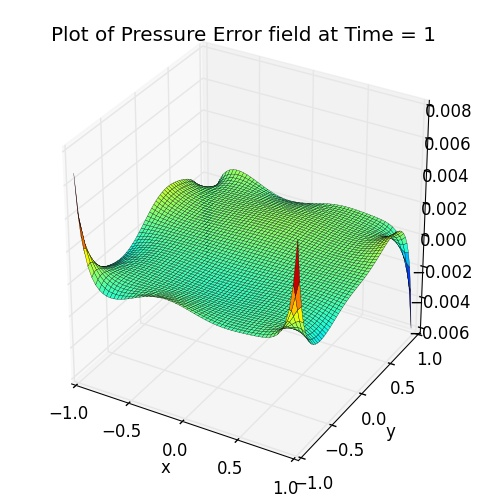
\includegraphics[width=2.5in]{figures/Pm1b_pf2_P_error_t_1_grid_60 - Copy.jpg}
		\caption{Pressure error field at grid size of 60}\label{fig:6.19a}		
	\end{subfigure}
	\quad
	\begin{subfigure}[t]{2.5in}
		\centering
		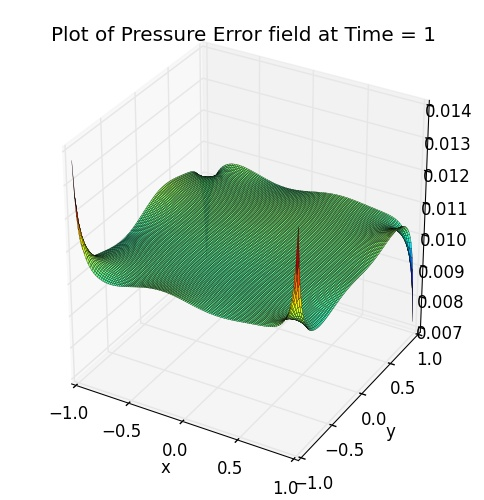
\includegraphics[width=2.5in]{figures/Pm1b_pf2_P_error_t_1_grid_120.jpg}
		\caption{Pressure error field at grid size of 120}\label{fig:6.19b}
	\end{subfigure}
	\caption{$3D$ surface plot of Pressure error fields for method $Pm\,1\,(b)$ on domain $[-1,1]^2$ at time = 1. A CFL number of 0.1 was used.}\label{fig:6.16}
\end{figure}

Therefore we infer that if we correct the numerical $\phi$ by subtracting the additional constant $a$ then we can recover the correct pressure solution. This requires an additional constraint being added to the Poisson equation to recover the unique $\phi$ solution. We call this new modified approach as ``Pressure normalisation".\\

Although not discussed in the literature of Projection methods, we infer that a normalisation process is also implemented in the literature by researchers.\\

There are many choices of normalisation. One common one is forcing the $\phi$ to satisfies an integral constraint:
\begin{equation}
\int_{\Omega}\,\int_{\Omega}\,\phi \,\,\, dx dy = 0
\end{equation}
\textbf{Is this right?}
However this approach involves calculating integrals and due to the limited timing we did not use it. This could be done in future researches.\\

Setting 
\begin{equation}
\phi^{n+1}_{nu} = \phi^{n+1}_{ex} + a
\end{equation}
where the subscripts ``nu" and ``ex" stands for numerical and exact solutions respectivelyBecause of non-uniqueness there is no ``exact" $\phi$ solution, here exact refers to the one required by the projection method. Other $\phi$ solutions would causing the pressure to converge differently as we have seen before.\\

In practice $\phi^{n+1}_{nu}$ is first solved using the Poisson equation with the zero Neumann boundary condition\\

Because the Poisson equation with Neumann boundary condition does not guarantee uniqueness of $\phi$, hence we need to think what other constraints it must satisfy in the projection methods. In turns out that $\phi$ satisfies the pressure update equation! Rearrange equation (11) we obtain an expression for the constant $a$:
\begin{equation}
a = \phi^{n+1}_{nu} - \dfrac{1}{Re} \nabla \cdot \textbf{u}^* + (p^{n+1/2} - p^{n-1/2})
\end{equation}

This requires the knowledge of $p^{n+1/2}$ which of course we don't have when solving for $\phi^{n+1}$! However remember that $a$ is just a constant added to $\phi$ (and pressure), hence if we know the the pressure field at one point in domain then we can fully recover $a$. This point is arbitrary, but in practice, it is usually chosen along the boundary or center or any other points easily accessed. Therefore we need to impose a ``partial" Dirichlet condition on pressure. It is partial because we only require the knowledge of point in space. In this section, we have chosen the point from the boundary.

\begin{equation}
a = \phi^{n+1}_{nu}\,(x,y)|_{(x,y)\in \partial\Omega} \,\,\,-\,\,\, \dfrac{1}{Re} \nabla \cdot \textbf{u}^*\,(x,y)|_{(x,y)\in \partial\Omega}\,\,\, +\,\,\, (p^{n+1/2} - p^{n-1/2})\,(x,y)|_{(x,y)\in \partial\Omega}
\end{equation}

Practically in order to ensure consistency we take 2 to 4 points along each boundary or corner and taking their average. \\

For the forced flow example we are considering, the analytical solution ($p = \sin(t)\cos(\pi x)\sin(\pi y)$) indicates the North and South boundaries ($y=\pm 1$) are essentially zero for domain $[-1,1]^2$. Therefore naturally one can consider inhomogeneous Dirichlet boundary condition for pressure variable. Then by picking one arbitrary point along the boundary (for instance $y=1$ and $x$ is arbitrary) our equation for $c$ reads:
\begin{equation*}
a = \phi^{n+1}_{nu}\,(x,1) \,\,\,-\,\,\, \dfrac{1}{Re} \nabla \cdot \textbf{u}^*\,(x,1)
\end{equation*}
In the case of Staggered grids the spatial point $(x,1)$ corresponds to an index of $i, \, j = \dfrac{1}{2}$ where $i$ stands for the horizontal index and $j$ the vertical index. Dropping the time index for convenience we obtain:
\begin{equation*}
a = \phi^{nu}_{i,\,1/2} \,\,\,-\,\,\, \dfrac{1}{Re} \nabla \cdot \textbf{u}^*_{i,\,1/2}
\end{equation*}

However in Staggered grids, the coordinate ($i,\,1/2$) is along the top edge of the grid and no pressure is stored at this point (pressure is stored at ($i,\,j$) locations). Therefore interpolation from nearby cells are needed. This introduces spatial interpolation error and hence care must be taken to avoid accumulation of spatial errors.\\

In this case, we use a 3rd order cubic interpolation for $\phi^{nu}_{i,\,1/2}$ from 3 nearby points: $\phi^{nu}_{i,\,1}$, $\phi^{nu}_{i,\,2}$ and $\phi^{nu}_{i,\,3}$. Cubic interpolation is needed to ensure the first order derivative of $\phi^{nu}_{i,\,1/2}$ is also second order accurate along the boundary.\\
We Taylor expand $\phi^{nu}_{i,\,1}$, $\phi^{nu}_{i,\,2}$ and $\phi^{nu}_{i,\,3}$ at location ($i,\,1/2$) up to order $\mathcal{O}(\Delta t^3)$ and we obtained an interpolation formula for $\phi^{nu}_{i,\,1/2}$ as

\begin{equation}
\phi^{nu}_{i,\,1/2} = \dfrac{15}{8}_{i,1} - \dfrac{5}{4}_{i,\,2}+\dfrac{3}{8}_{i,\,3}
\end{equation}
Exactly the formula can be used for $\nabla \cdot \textbf{u}^*$ since they are stored at the same locations as $\phi$.\\

Then the exact $\phi^{n+1}$ can thus be obtained by subtracting $c$ from $\phi^{n+1}_{nu}$ point-wisely. Thus we minus the same constant $a$ on every point of $\phi^{nu}$. Then the correct pressure can be recovered and we call it the ``Normalised Pressure". This in theory should fix the problem of error of error enlargement at finer grids. And this method indeed works as we shall shortly!\\

For Projection method $Pm\,2$, exactly the process is used. In fact the expression for $c$ is identical.\\

For Gauge method, exactly the same procedure can be implemented too. From solving the Poisson equation we know that:
\begin{equation}
\chi^{n+1}_{nu} = \chi^{n+1}_{ex} + b\,\,\,\text{ and }\,\,\,\chi^{n}_{n} = \chi^n_{ex} + c
\end{equation}
where $b$ and $c$ are constants. They are generally not equal and hence Gauge method also suffers from the non-uniqueness problem.\\

Again the point where we evaluate $b$ and $c$ is arbitrary, so let's use the same one considered above.\\
Substitute the expression of $\chi_{nu}$ into the pressure update equation and rearranging we obtain:
\begin{equation}
b - c = \chi^{n+1,\,\,\,nu}_{i,\,1/2} - \chi^{n,\,\,\,nu}_{i,\,1/2} + \dfrac{\Delta t}{2\,Re}(\nabla \cdot m^{n+1}_{i,\,1/2} + \nabla \cdot m^n_{i,\,1/2})
\end{equation}
